\documentclass[12pt]{book}

\usepackage{url}
\usepackage{amssymb,amsthm}
\usepackage{graphicx,color}

\usepackage{longtable}

\usepackage{balance}

\usepackage{cite}
\usepackage{amsmath}
\usepackage{amssymb}

\usepackage{color, colortbl}
\usepackage{times}
\usepackage{caption}
\usepackage{rotating}
\usepackage{subcaption}
\usepackage{mathtools}

\usepackage{setspace}

\usepackage{listings}


\usepackage{python}

\usepackage[T2A]{fontenc}
\usepackage[utf8]{inputenc}
\usepackage{bm}

\usepackage[Sonny]{fncychap}

\usepackage{geometry}

\newtheorem{theorem}{Теорема}
\newtheorem{example}{Пример}
\newtheorem{definition}{Определение}
\newtheorem{lemma}{Лемма}

\renewcommand{\chaptername}{Глава}
\renewcommand{\contentsname}{Оглавление}
\renewcommand{\bibname}{Литература}
\renewcommand{\tablename}{Таблица}
\renewcommand{\figurename}{График}

\newcommand{\XXXnote}[1]{{\bf\color{red} XXX: #1}}
\newcommand{\YYYnote}[1]{{\bf\color{red} YYY: #1}}
\newcommand*{\etal}{{\it et al.}}

\newcommand{\eat}[1]{}
\newcommand{\bi}{\begin{itemize}}
\newcommand{\ei}{\end{itemize}}
\newcommand{\im}{\item}
\newcommand{\eg}{{\it e.g.}\xspace}
\newcommand{\ie}{{\it i.e.}\xspace}
\newcommand{\etc}{{\it etc.}\xspace}

\newcommand{\ccb}{\cellcolor{blue}}
\newcommand{\ccl}{\cellcolor{lightblue}}
\newcommand{\ccr}{\cellcolor{red}}

\definecolor{blue}{rgb}{0.48,0.7,0.98}
\definecolor{lightblue}{rgb}{0.85,1,1}
\definecolor{red}{rgb}{0.76,0.23,0.23}

\def\P{\mathop{\mathsf{P}}}
\def\E{\mathop{\mathsf{E}}}



\begin{document}

\sloppy
%\title{Python в алгоритмах для детей и взрослых}
%\author{Written by artificial intelligence}
%\maketitle

\begin{titlepage}
\newgeometry{left=7.5cm} %defines the geometry for the titlepage
\pagecolor{red}
\noindent
%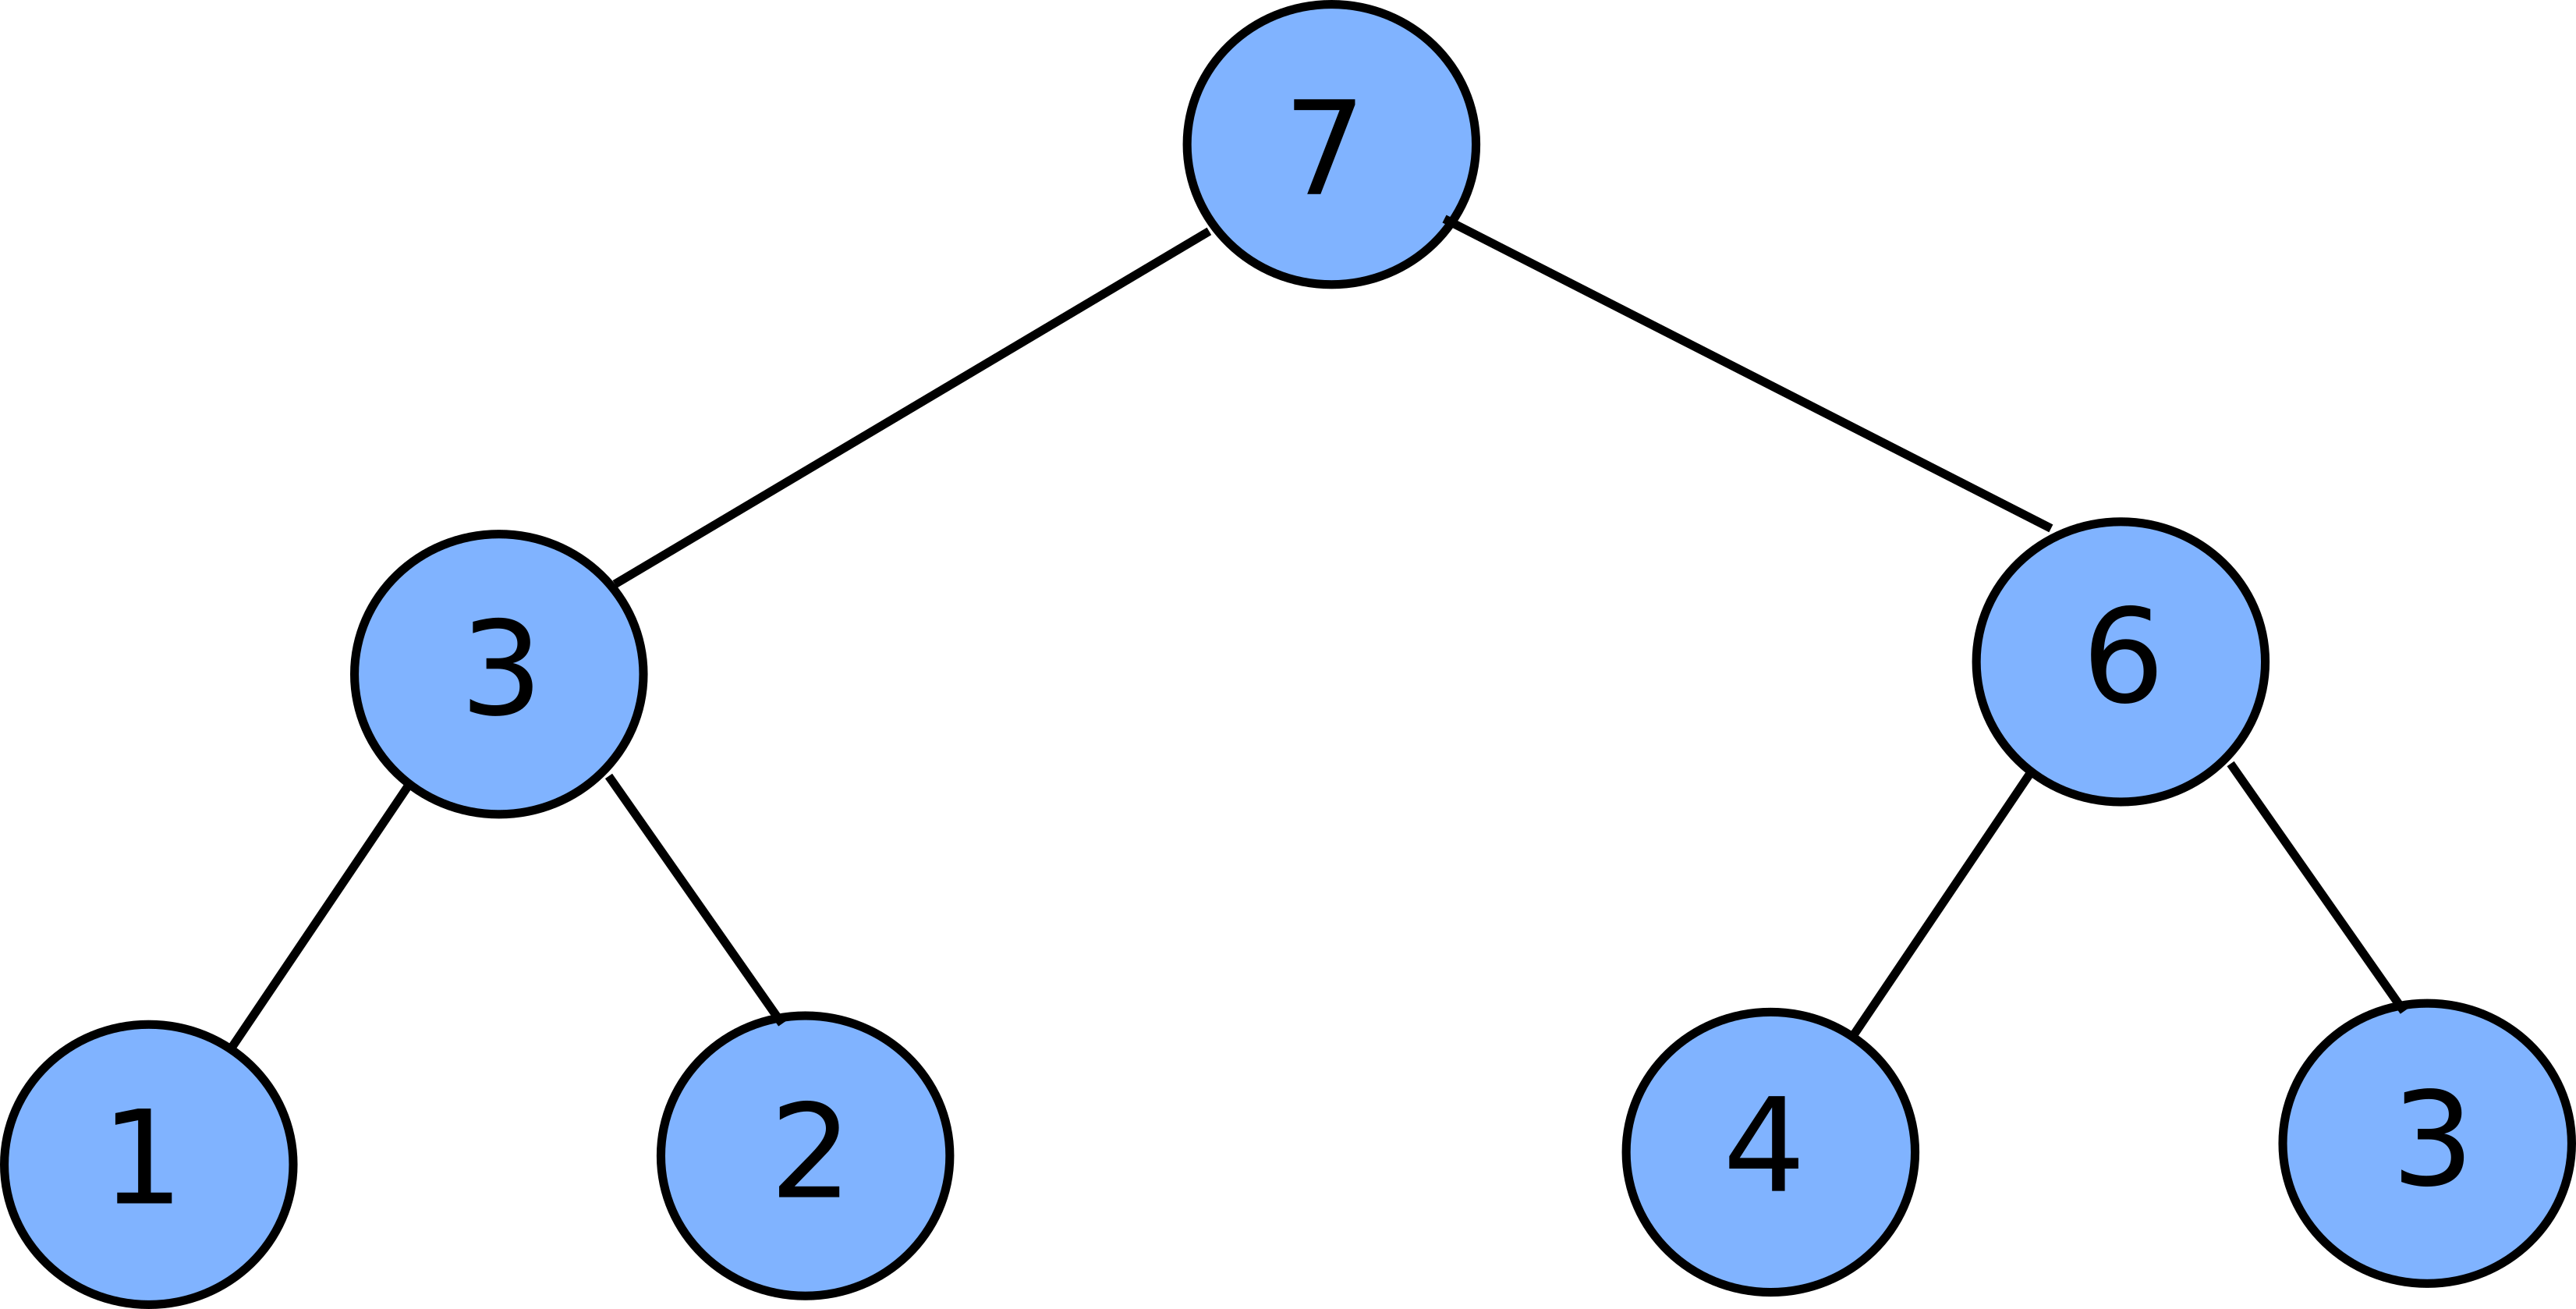
\includegraphics[width=5cm]{graphics/binary_tree.png}\\[20em]
\noindent\\[10em]
{\huge \textsf{Python в примерах для детей и взрослых}}
\vskip\baselineskip
\noindent
\vfill
\color{white}
\makebox[0pt][l]{\rule{1.3\textwidth}{1pt}}
\par
\noindent
\textbf{\textsf{Дмитрий Купцов}}
\par
\noindent
\textsf{2020}
\end{titlepage}
\restoregeometry % restores the geometry
\nopagecolor% Use this to restore the color pages to white

\tableofcontents


\input intro.tex
%\input background.tex
%\input data.tex
%\input preprocess.tex
%\input metrics.tex
%\input solution.tex
%\input conclusions.tex

\bibliographystyle{abbrv}
\bibliography{mybib}

\end{document}



